\begin{center}
\indent
\textit{La loro teoria serve ad inquadrare la risoluzione dei sistemi di equazioni lineari. \\ Spazio vettoriale delle matrici, spazio vettoriale delle $n$-uple di numeri reali.}
\end{center}

\section{Spazi vettoriali su un campo $\field$}

Uno spazio vettoriale \`e una struttura algebrica $(V, +, \cdot)$ su un campo $\field$ le cui operazioni sono $+ : V \times V \to V$ e l'operazione ``esterna'' $\cdot : \field \times V \to V$. Il $\cdot$ \`e detto ``moltiplicazione esterna''. Gli elementi di $V$ si dicono \textit{vettori}.

Uno spazio vettoriale gode delle seguenti propriet\`a:
\begin{description}
    \item[1V] $(V, +)$ \`e un gruppo abeliano
    \item[2V] $\forall k \in \field$, $\forall v, w \in V$, $k \cdot (v + w) = k \cdot v + k \cdot w$. Questa propriet\`a \`e detta distributiva rispetto all'addizione in $V$ (ossia, rispetto all'addizione vettoriale).
    \item[3V] $\field$ \`e un campo, quindi $\forall k, h \in \field$ e $\forall v \in V$, $(k + h) \cdot v = k \cdot v + h \cdot v$. Questa propriet\`a \`e detta distributiva rispetto all'addizione in $\field$
    \item[4V] $\forall k, h \in \field$, $\forall v \in V$, $(h \cdot k ) \cdot v = h \cdot (k \cdot v) = k \cdot (h \cdot v)$. \`E una specie di propriet\`a associativa.
    \item[5V] $\forall v \in V$, $1 \cdot v = v$
\end{description}

Un elemento $k \in \field$ viene detto ``scalare''.

Gli spazi vettoriali danno una veste teorica alla risoluzione dei sistemi lineari.

\subsubsection{Esempi di spazi vettoriali}

Il nome degli spazi vettoriali viene dagli spazi vettoriali geometrici. $(V_O, +, \cdot)$ \`e lo spazio vettoriale su $\reals$ dei vettori dello spazio euclideo applicati in un punto $O$ (detto ``origine'').

La somma fra vettori geometrici si effettua con la ``regola del parallelogramma'' (figura \ref{fig:parallelogramma}). Le forze possono essere rappresentate dai vettori del piano.

\begin{figure}[ht]
\centering
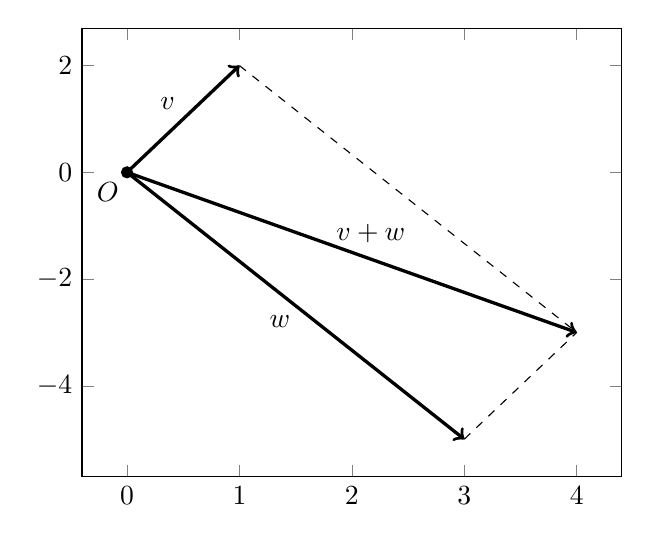
\begin{tikzpicture}
\begin{axis}[
    % graph options
]
\addplot [black, mark = *, nodes near coords=$O$,every node near coord/.style={anchor=45}] coordinates {( 0, 0)};
\addplot [black, nodes near coords=$v$,every node near coord/.style={anchor=315}] coordinates {( 0.5, 1)};
\addplot [black, nodes near coords=$w$,every node near coord/.style={anchor=45}] coordinates {( 1.5, -2.5)};
\addplot [black, nodes near coords=$v+w$,every node near coord/.style={anchor=225}] coordinates {( 2, -1.5)};
\addplot[very thick,->] coordinates {(0,0) (1,2)};
\addplot[very thick,->] coordinates {(0,0) (3,-5)};
\addplot[very thick,->] coordinates {(0,0) (4,-3)};
\addplot[dashed] coordinates {(1,2) (4,-3)};
\addplot[dashed] coordinates {(3,-5) (4,-3)};
\end{axis}
\end{tikzpicture}
\caption{\label{fig:parallelogramma}Metodo del parallelogramma}
\end{figure}

L'elemento neutro \`e il vettore nullo, i cui estremi coincidono in $O$, e si indica con $\underline{\underline{O}} = \overrightarrow{OO}$.  L'inverso di un vettore $v$ \`e chiamato $-v$, ha stessa direzione, stesso modulo e verso contrario.

Per creare lo spazio vettoriale abbiamo bisogno infine dell'operazione esterna: il prodotto scalare $ \cdot : \reals \times V \to V$ (figura \ref{fig:prodotto_scallare}).

\begin{figure}[ht]
\centering
\begin{tikzpicture}
\begin{axis}[
    % graph options
]
\addplot [black, mark = *, nodes near coords=$O$,every node near coord/.style={anchor=135}] coordinates {( 0, 0)};
\addplot [black, nodes near coords=$v$,every node near coord/.style={anchor=315}] coordinates {( 0.5, 1)};
\addplot [black, nodes near coords=$-v$,every node near coord/.style={anchor=315}] coordinates {( -0.5, -1)};
\addplot [black, nodes near coords=$2v$,every node near coord/.style={anchor=135}] coordinates {( 1.5, 3)};
% \addplot[only marks] coordinates {(0,0)}; % punto
\addplot[very thick,->] coordinates {(0,0) (1,2)};
\addplot[dashed,->] coordinates {(0,0) (-1,-2)};
\addplot[dashed,->] coordinates {(0,0) (2,4)};
\end{axis}
\end{tikzpicture}
\caption{\label{fig:prodotto_scallare}Prodotto scalare}
\end{figure}

Le $n$-uple degli elementi di un campo $\field$ sono uno spazio vettoriale, ossia $(\field^n, +, \cdot)$ \`e uno spazio vettoriale su $\field$. Se ad esempio il campo \`e $\reals$ e $n = 3$, prendiamo le terne di numeri reali $(a,b,c) \in \reals^3$. La somma di due terne \`e $(a,b,c) + (x,y,z) = (a + x, b + y, z + c)$. Moltiplicare una terna per un numero si chiama ``moltiplicare per uno scalare'', e $r \cdot (a,b,c) = (r \cdot a, r \cdot b, r \cdot c)$.

Anche i polinomi $(\field[x], +, \cdot)$ sono uno spazio vettoriale. Moltiplicare un polinomio per uno scalare (ossia per un elemento del campo) vuol dire moltiplicare tutti i coefficienti per lo scalare.

Abbiamo poi visto lo spazio vettoriale delle matrici. L'insieme delle matrici $(\matrices_{m \times n} (\field), +, \cdot)$ \`e uno spazio vettoriale. Date due matrici $A = (a_{i,j})$ e $B = (b_{i,j})$, la loro somma \`e $A + B = (a_{i,j} + b_{i,j})$, mentre la moltiplicazione per uno scalare $k$ \`e $k \cdot A = (k \cdot a_{i,j})$.

Dato un sottocampo di un campo $\subfield \subseteq \field$, ad esempio $\rationals \subseteq \reals \subseteq \complexes$, possiamo vedere $\field$ come spazio vettoriale su $\subfield$. % diceva: possiamo vedere $\subfield$ come sottocampo di $\field$. ma credo intendesse questo che ho scritto
$(\field, +, \cdot)$ ha l'operazione $\cdot : \subfield \times \field \to \field$, che dati $h \in \subfield$ e $ k \in \field \mapsto h \cdot k$.

\subsection{Sottospazi vettoriali}

Un sottoinsieme $W \subseteq V$, con $(V, +, \cdot)$ a indicare uno spazio vettoriale, si dice sottospazio di $V$ se $(W, +, \cdot)$ \`e ancora uno spazio vettoriale. Le operazioni devono essere $+ : W \times W \to W$, e $\cdot : \field \cdot W \to W$.

Condizione necessaria e sufficiente affinch\'e un insieme $W \subseteq V$ sia un sottospazio di $(V, +, \cdot)$ \`e che $W \neq \emptyset$, $\nullelement \in W$, e che:
\begin{align*}
\forall v, w \in W &\implies (v - w) \in W \\
\forall k \in \field , \, \forall w \in W &\implies k \cdot w \in W
\end{align*}

% Se $W$ \`e un sottospazio di $V$, (W, +) deve essere un sottogruppo di (V, +) \iff se prendo due vettori v, w \in W \implies (v - w) \in W. Poi bisogna vedere che \forall k \in \field e \forall w \in W \implies k \cdot w \in W. Quindi condizione necessaria e sufficiente affinch\'e un insieme W \subseteq V sia un sottospazio \`e che se W \neq \emptyset e \nullelement \in W, W deve verificare tutta la roba sopra.

Nello spazio dei vettori geometrici, quali sono i sottospazi? Deve contenere il vettore nullo. Quindi $W_0 = \{ \nullelement \}$ \`e un sottospazio banale. Se il sottospazio $W_1$ contiene un vettore $v \neq \nullelement$, deve contenere anche:
\begin{itemize}
    \item $0_{\field} \cdot v = \nullelement \in W_1$. Infatti $0_{\field} \cdot v = (0_{\field} + 0_{\field}) \cdot v = 0_{\field} \cdot v + 0_{\field} \cdot v \implies 0_{\field} \cdot v = \nullelement$
    \item $-1 \cdot v = - \cdot v$. Infatti $v + (-1) \cdot v = (1 - 1) \cdot v = 0_{\field} \cdot v = \nullelement$. Se moltiplico un vettore per $-1$ ottengo il suo opposto.
    \item deve contenere tutti i multipli $k \cdot v$, con $k \in \reals$.
\end{itemize}
Questo \`e un sottospazio, infatti verifica che $\forall v, w \in W_1 \implies v - w \in W_1$, e abbiamo visto che $\forall k \in \reals$, $k \cdot v \in W_1$.
\[
W_1 = \{ k \cdot v \in V : k \in \reals \}
\]
Un sottospazio quindi \`e il sottospazio dei vettori che hanno la stessa direzione di $v$, ossia \`e il sottospazio dei multipli di un vettore. Un sottospazio che contiene un vettore deve per forza contenere tutti i suoi multipli.

Vediamo cosa succede se il sottospazio contiene un vettore $w \neq k \cdot v$ con $k \in \reals$. Deve contenere anche tutti i multipli di $w$, per quanto appena visto. E deve quindi contenere le somme di tutti i vettori multipli di $v$ e di tutti i vettori multipli di $w$.
\[
W_2 = \{ a \cdot v + b \cdot w : a, b \in \reals \text{ e } v \neq k \cdot w \}
\]
$W_2$ sono tutti i vettori sul piano individuato dai vettori $v$ e $w$.

% disegnare vettore v, suo opposto, punto O, vettore w, direzione di v

Se aggiungiamo un terzo vettore diverso da $k \cdot v$ e $h \cdot w$ con $h, k \in \reals$, abbiamo che lo spazio vettoriale $W_3 \supseteq W_2$ \`e o $W_3 = W_2$ o $W_3 = V$. $W_2$ \`e detto ``massimale''.

Non esiste un sottospazio che lo contenga propriamente e che \`e diverso da tutto lo spazio.

Prendiamo l'insieme dei polinomi tali per cui il grado di $p(x) = n$.
\[
W_1 = \{ p(x) : \delta (p(x)) = n \}
\]
Non \`e un sottospazio: non contiene il polinomio nullo, e la differenza fra due polinomi non sempre ha grado $n$.
\[
W_2 = \{ p(x) : \delta (p(x)) \le n \}
\]
Questo \`e invece un sottospazio.
\[
W_3 = \{ p(x) : \delta (p(x)) \le 3 \text{ e } a_1 = a_2 = 0 \}
\]
Anche questo \`e un sottospazio. $\nullelement \in W_3$. La differenza fra due polinomi $a_0 + a_3 \cdot \cdot x^3 - b_0 - b_3 \cdot x^3 = a_0 - b_0 + (a_3 - b_3) \cdot x^3$ \`e ancora dentro $W_3$, quindi \`e un sottogruppo. Inoltre $k \cdot (a_0 + a_3 \cdot x^3)$ \`e $k \cdot a_0 + k \cdot a_3 \cdot x^3$, che \`e sempre in $W_3$.

Consideriamo ora $(\reals^4, +, \cdot)$, e il sottoinsieme:
\[
W = \{ (a_1, a_2, a_3, a_4) : a_1 + a_2 = 0 \}
\]
Prendiamo due elementi $(a_1, a_2, a_3, a_4)$ e $(b_1, b_2, b_3, b_4)$ e facciamo la differenza, ossia $(a_1 - b_1, a_2 - b_2, a_3 - b_3, a_4 - b_4)$. Vediamo che $a_1 - b_1 + a_2 - b_2$ \`e uguale a 0. Per verificare che \`e un sottospazio, dobbiamo verificare che una quaterna moltiplicata per $k$ \`e ancora dentro $W$.
\[
k \cdot (a_1, a_2, a_3, a_4) = (k \cdot a_1, k \cdot a_2, k \cdot a_3, k \cdot a_4)
\]
\`E verificato, infatti $k \cdot a_1 + k \cdot a_2 = k \cdot (a_1 + a_2) = k \cdot 0 = 0$.

\`E importante controllare sempre che il sottospazio sia vuoto, e che contenga il vettore nullo.
\[
W_1 = \{ (a_1, a_2, a_3, a_4) : a_1 = a_2^2 \}
\]
Questo non \`e un sottospazio, infatti non verifica che $k \cdot a_1 = k \cdot a_2^2$ , essendo $(k \cdot a_2)^2$.

Consideriamo lo spazio vettoriale delle matrici quadrate $(\matrices_2 (\reals), +, \cdot)$.
\[
W = \left\{ 
\begin{smallpmatrix}
a & b  \\
c & d 
\end{smallpmatrix}
: a = 0 \right\}
\]
\`E un sottospazio, infatti $\nullelement = \begin{smallpmatrix}0&0\\ 0&0\end{smallpmatrix} $ \`e dentro $W$. Inoltre:
\[
k \cdot 
\begin{pmatrix}
0 & b \\
c & d
\end{pmatrix}
=
\begin{pmatrix}
0 & k \cdot b \\ 
k \cdot c & k \cdot d
\end{pmatrix}
\]
Consideriamo l'insieme:
\[
W_1 = \left\{
\begin{smallpmatrix}
a & b \\
c & d 
\end{smallpmatrix}
: a = d - 1 \right\} 
\]
Non \`e un sottospazio, poich\'e $\nullelement \notin W_1$.

\begin{prop}[Proposizione fondamentale per gli spazi vettoriali]
Siano $U, W$ sottospazi di $V \implies U \cap W$ \`e un sottospazio di $V$.
\end{prop}
Questo vale per tutte le strutture algebriche.

\begin{proof}
Vediamo che $\nullelement \in U \cap W$, essendo contenuto in entrambi.

Sia $v, w \in U \cap W \implies v - w \in U \cap W$, essendo $v - w \in U e v - w \in W$.

Analogamente se $v \in U \cap W$ e $k \in \field \implies k \cdot v \in U \cap W$, essendo $U$ e $W$ sottospazi e quindi essendo ogni multiplo di $v$ in entrambi.
\end{proof}

\subsection{Reticolo dei sottospazi vettoriali}

Con i sottospazi vettoriali abbiamo un altro esempio di reticolo.

$\subgroupset(V)$ \`e l'insieme dei sottospazi dello spazio vettoriale $(V, +. \cdot)$. $(\subgroupset(V), \subseteq)$ \`e un reticolo, e $\subseteq$ indica la relazione di sottospazio. Siano $U, W \subseteq V$, l'$\inf$ di $U$ e $W$ \`e $U \cap W = U \infop W$. Verifica le propriet\`a dell'$\inf$, infatti se $T \subseteq U, W \implies T \subseteq U \cap W$.

Abbiamo gi\`a visto con i sottogruppi che l'unione di due sottogruppi in generale non \`e un sottogruppo. Anche qui, l'unione di due sottospazi non \`e, in generale, un sottospazio.

Abbiamo visto ad esempio che due sottospazi di $(V_O, +, \cdot)$ contenenti ciascuno i multipli di un solo vettore hanno un'unione che non \`e un sottospazio.

Il $\sup$ di $U$ e $W$, $U \supop W$, deve contenere l'unione di $U$ e $W$.
\[
U \subseteq U \cup W \subseteq U \supop W
\]
Inoltre sia $T$ un sottospazio di $V$ che contiene sia $U$ che $W$, $U, W \le T \implies U \supop W \le T$.

Quindi il $\sup$ \`e il pi\`u piccolo dei sottospazi che contiene l'unione. Quindi \`e l'intersezione di tutti i sottospazi che contengono sia $U$ che $W$.
\[
U \supop W = \bigcap_{U, W \subseteq T} T
\]
Vediamo come si caratterizza il $\sup$.

Abbiamo il reticolo dei sottospazi di uno spazio vettoriale.

Prendiamo un sottoinsieme $S$ dello spazio vettoriale $V$. Definiamo il sottospazio generato da da $S$. Lo indichiamo con $\pow{S}$. \`E definito come il pi\`u piccolo dei sottospazi contenenti $S$. $U \supop W$ \`e il sottospazio generato da $\pow{U \cup W}$.

Il sottospazio generato da $S$ \`e quindi:
\[
\pow{S} = \bigcap_{S \subseteq T} T
\]
Ossia l'intersezione di tutti i sottospazi contenenti $S$.

Prendendo $v \in V_O$, il sottospazio generato da $v$ \`e:
\[
\pow{v} = 
\begin{cases}
\nullelement \text{ se } v = \nullelement \\
\{ k \cdot v : k \in \field \} \text{ se } v \neq \nullelement
\end{cases}
\]

\subsection{Combinazioni lineari e indipendenza lineare}

Negli spazi vettoriali ci sono due concetti fondamentali da capire se si vuole capire qualcosa. Fissateli bene a mente, coglione.

\begin{description}
    \item[Combinazione lineare] Dati n vettori $v_1, \dots v_n$ vettori in $V$, e $n$ scalari $k_1, \dots k_2 \in \field$, la combinazione lineare dei vettori $v_1 \dots v_n$ \`e un vettore:
    \[
    v = k_1 \cdot v_1 + \dots + k_n \cdot v_n
    \]
    Le combinazioni lineari di un solo vettore $v$ sono tutti i multipli del vettore $v$.
    \item[Indipendenza lineare] \textit{DA DEFINIRE!}
\end{description}

\subsection{Esempi di combinazioni lineari}

Se prendiamo lo spazio vettoriale $(\reals^2, +, \cdot)$, un vettore qualunque $(a,b$) possiamo scriverlo come combinazione lineare dei vettori $(1,0)$ e $(0,1)$.
\[
(a,b) = a \cdot (1, 0) + b \cdot (0, 1)
\]
Un vettore di $\reals^3$ \`e formato da tutte le combinazioni lineari dei vettori $(1,0,0)$, $(0,1,0)$ e $(0,0,1)$.

In generale, un vettore di $\reals^n$ \`e formato dalla combinazione lineare di tutti i vettori $e_1 \dots e_n$ dove:
\[
e_i =
\begin{cases}
1 \text{ al posto } i \\
0 \text{ altrimenti}
\end{cases}
\]
Nello spazio dei polinomi $\reals[x]$, un polinomio $p(x)$ \`e combinazione lineare dei polinomi $\{ 1, x, x^2, \dots x^n, \dots \}$, ossia combinazione lineare dei polinomi $\{ x^i : i \in \naturals \}$.

Consideriamo le matrici quadrate di ordine 2, $\matrices_2 (\reals)$. Ogni matrice $\begin{smallpmatrix}a&b \\ c&d\end{smallpmatrix}$ \`e una combinazione lineare del tipo:
\[\
a \cdot
\begin{pmatrix}
1 & 0 \\
0 & 0 
\end{pmatrix}
+ b 
\begin{pmatrix}
0 & 1 \\
0 & 0 
\end{pmatrix}
+ c 
\begin{pmatrix}
0 & 0 \\
1 & 0 
\end{pmatrix}
+ d 
\begin{pmatrix}
0 & 0 \\
0 & 1
\end{pmatrix}
\]
Tutte le matrici nello spazio delle matrici quadrate di ordine 2 sono combinazione lineare delle matrici $\begin{smallpmatrix}1&0 \\ 0&0\end{smallpmatrix}$, $\begin{smallpmatrix}0&1 \\ 0&0\end{smallpmatrix}$, $\begin{smallpmatrix}0&0 \\ 1&0\end{smallpmatrix}$, $\begin{smallpmatrix}0&0 \\ 0&1\end{smallpmatrix}$.

In generale, tutte le matrici $\matrices_{m \times n} (\reals)$ sono combinazioni delle matrici $E_{h,k} (a_{i,j})$ dove:
\[
a_{i,j} = 
\begin{cases}
1 \text{ se } i = h \text{ e } j = k \\
0 \text{ altrimenti}
\end{cases}
\]
Nel caso di prima delle matrici quadrate di ordine 2, le matrici sono $E_{1,1}, E_{1,2}, E_{2,1}, E_{2,2}$.

Ritroviamo le combinazioni lineari negli spazi generati da sottoinsiemi di uno spazio vettoriale. $S$ \`e sottoinsieme dello spazio $(V, +, \cdot)$. $\Sigma (S)$ \`e insieme delle combinazioni lineari dei vettori di $S$. Quindi ogni $v \in \Sigma(S)$ \`e una combinazione lineare del tipo $v = a_1 s_1 + \dots + a_n s_n$ con $s_i \in S$.

\begin{prop}
$\pow{S}$, ossia lo spazio generato da $S$, \`e proprio $\Sigma(S)$.
\end{prop}
\begin{proof}
Si dimostra per doppia inclusione. Banalmente $S \subseteq \Sigma(S)$, e $\Sigma(S)$ \`e un sottospazio di $V$. Infatti la differenza di due combinazioni lineari \`e in $\Sigma (S)$, cos\`i come il prodotto scalare di una combinazione lineare. Quindi $\pow{S} \subseteq \Sigma (S)$.

Dobbiamo far vedere che ogni combinazione lineare \`e contenuta in $\pow{S}$.
\[
v \in \Sigma(S) \implies v = a_1 \cdot s_1 + \dots a_n \cdot s_n \text{ con } s_i \in S
\]
$S$ \`e sottoinsieme di $T$, con $T$ sottospazio di $V$. $s_i \in T \forall i$, $a_i \cdot s_i \in T \forall i \implies v \in T$. $\Sigma(S) \subseteq T \forall T$ tale che $S \subseteq T$.
\end{proof}

Abbiamo quindi un'altra definizione del $\sup$ di due sottospazi.
\[
U \supop W = \pow{U \cup W} = \Sigma(U \cup W) = \bigcap{U \cup W \subseteq T} T
\]
\begin{prop}
\[
(U \supop W) = U + W
\]
$U + W$ \`e l'insieme di tutti i vettori che posso scrivere come somma di $u + w$ con $u \in U$ e $w \in W$.
\[
U + W = \{ u + w : u \in U \text{ e } w \in W \}
\]
\end{prop}
\begin{proof}
Banalmente $U + W \subseteq \Sigma(U \cup W)$, ossia $U + W$ sono combinazioni lineari degli elementi di $U$ e $W$ in cui i coefficienti delle combinazioni lineari sono sempre 1.

Abbiamo anche che $U$ e $W \subseteq U + W$, che risulta essere un sottospazio.

Infatti prendendo gli elementi $(u + w)$ e $(u' + w')$, $(u + w) - (u' + w') = (u - u') + (w - w')$ \`e ancora in $U + W$. Poi $k \cdot (u + w) = k \cdot u + k \cdot w$ \`e dentro $U + W$.

Quindi se $U, W \subseteq U + W$, ed essendo $\Sigma(U \cup W)$ il pi\`u piccolo dei maggioranti di $U$ e $W$, deve essere che $U + W = \Sigma(U \cup W)$.
\end{proof}
\begin{prop}[Somma diretta fra spazi vettoriali]
$W$ e $U$ hanno somma diretta, che si indica con $U \oplus W$, se $ U \cap W = \{ \nullelement\}$. Le seguenti proposizioni sono equivalenti:
\begin{enumerate}
    \item\label{somma_diretta_1} $U$ e $W$ hanno somma diretta
    \item\label{somma_diretta_2} ogni vettore di $U + W$ si pu\`o esprimere in un unico modo come $u + w$, con $u \in U$ e $w \in W$
\end{enumerate}
\end{prop}
\begin{proof}
Il punto \ref{somma_diretta_1} implica il punto \ref{somma_diretta_2}.

Sia $v \in U + W$ tale che $v = u + w = \bar{u} + \bar{w}$, allora $u = \bar{u}$ e $w = \bar{w}$.

Infatti $(u + w) - (\bar{u} + \bar{w}) = \nullelement$. Da questo segue che possiamo scrivere $(u - \bar{u}) + (w - \bar{w}) = \nullelement$. Quindi $u - \bar{u} = - (w - \bar{w})$. Questo vettore si pu\`o scrivere come somma di due elementi di $U$ e come somma di due elementi di $W$, quindi \`e nell'intersezione. Quindi \`e il vettore nullo $\nullelement$, e quindi $u = \bar{u}$ e $w = \bar{w}$.

Ora vediamo che il punto \ref{somma_diretta_2} implica il punto \ref{somma_diretta_1}.

Dobbiamo dimostrare che l'intersezione contiene solo il vettore nullo. $U \cap W = \{ \nullelement \}$.

Consideriamo $v \in U \cap W$. Se $v \neq \nullelement$, dobbiamo scriverlo come somma di due vettori in $U$ e in $W$ in due modi diversi, cos\`i andiamo in contraddizione con l'ipotesi del punto \ref{somma_diretta_2}.

$v = \nullelement + v$ con $v \in W$, e $v = v + \nullelement$ con $v \in U$. Contraddizione.
\end{proof}

% SONO ARRIVATO QUI A CONTROLLARE

% SONO ARRIVATO QUI A SCRIVERE

\section{Sistemi lineari}

Un sistema lineare \`e un'equazione lineare in $n$ variabili.

\[
a_1 x_1 + a_2 x_2 + \dots + a_n x_n = b
\]

Un sistema lineare \`e un insieme di equazioni lineari nello stesso numero di variabili.

$a_1, a_2, \dots, a_n, b \in \reals$. $a_1, a_2, \dots, a_n$ sono i coefficienti, $b$ \`e il termine noto.

$x_1, x_2, \dots, x_n$ sono chiamate variabili.

\[
3x_1 - 2x_2 + x_4 = 3
\]

Equazione lineare in 4 variabili. I coefficienti sono $(3, -2, 0, 1)$. Il termine noto \`e 3.

La soluzione di un'equazione in $n$ variabili \`e una $n$-upla $(s_1, s_2, \dots, s_n)$ con $s_1, s_2, \dots, s_n \in \reals$ t.c. se sostituita al posto delle variabili rende l'equazione un'identit\'a: $a_1 s_1 + a_2 s_2 + \dots a_n s_n = b$.

Risolvere un sistema lineare vuol dire trovare tutte le $n$-uple che soddisfano le equazionin del sistema.
















